\chapter{Results}

\noindent This study is built upon a robust computational framework, the consistency of which has been rigorously validated through a series of sanity checks, as portrayed in Section~\ref{sec:sanity_checks_results}. The simulation results for rain volumes, derived from the hydrometeor scattering model established in the previous chapter, are presented and analyzed in Section~\ref{sec:rain_volume_sims}. 

\section{Software sanity checks}
\label{sec:sanity_checks_results}

\noindent Testing the code requires knowing the expected outcome from a simulation. To check whether the principle of linearity is respected, an established interference phenomenon was reproduced (see Section~\ref{sec:single_slit}). Moreover, the coherence principle is verified when the RCS expected from a theoretically well-understood target is replicated as a sum of the contributions of its coherent scattering portions, this is detailed in Section~\ref{sec:thin_square_plate}.

\subsection{Single slit diffraction figure}
\label{sec:single_slit}

\noindent A well-known phenomenon is the single slit diffraction, which results in a figure for the electric field with a central maximum and many dimmer maxima on the sides. \\

\noindent This model, depicted in Figure~\ref{fig:diffraction_figure_drawing}, represents a slit as a line of 100 coherent secondary sources at the origin. A transmitter in the far-field is located at $-d$, and a screen of receivers, tuned to the transmitter's frequency, is positioned at $d$. The time-averaged electric field from a continuous monochromatic wave is computed across the receiver array. \\

\begin{figure}
	\centering
	\includegraphics[width=0.75\textwidth]{images/slit_drawing.png}
	\caption{Single slit diffraction simulation set-up. A transmitter, slit and set of receivers are aligned and sufficiently spaced, depending on the size of the slit (1 m) and the size of the wavelength (3 cm).}
	\label{fig:diffraction_figure_drawing}
\end{figure}

\noindent The theoretical formula for the intensity at the screen is:

\begin{equation}
	\label{eq:diffraction}
	I(\theta) = I_{0} \left[ \frac{\sin\left(\frac{ka\sin(\theta)}{2}\right)}{\frac{ka\sin(\theta)}{2}}\right]^{2}.
\end{equation}

\noindent The far-field region assumes $\lambda \ll d$. Therefore if the frequency is set to 10 GHz, a 3 cm wavelength signal is produced and $d = 1000$ m is sufficient to get the expected oscillating result illustrated in Figure~\ref{fig:diffraction_figure_plot}. \\

\begin{figure}
	\centering
	\includegraphics[width=0.8\textwidth]{images/plots/diffraction_figure_voltage.pdf}
	\caption{Result for a simulated slit diffraction phenomenon. The time-averaged electric field across the receiving array forms the interference figure.}
	\label{fig:diffraction_figure_plot}
\end{figure}

\noindent We can conclude that interference is well portrayed by the code.

\subsection{Thin square plate as a collection of coherent scattering regions}
\label{sec:thin_square_plate}

\noindent The RCS of many simple shapes is obtained mathematically as explained by Crispin and Maffet in Reference~\cite{crispinRadarCrosssectionEstimation1965}. In particular, a thin square plate was chosen for this work. \\

\noindent The expected backscatter RCS of a metallic thin square plate is:

\begin{equation}
	\sigma_{\text{RCS}} = \frac{4a^{4}}{\lambda^{2}}\left[\frac{\sin(ka \sin(\theta))}{ka\sin(\theta)}\right]^{2}.
\end{equation} 

\noindent The zenith angle $\theta$ defines the inclination of the incident/scattered ray respect to the vertical, and $a$ the size of the square's edge. The monostatic geometry is adopted here, since the formula above describes the backscatter effect. The simulation was carried out considering a thin parallelogram placed above the antennas. \\

\noindent In Figure~\ref{fig:square_drawing} is portrayed the sectioning of the parallelogram operated following a generic direction of the incident ray. For every inclination, the volume of every section was carefully calculated to obtain a faithful representation of the chosen shape.\\

\begin{figure}
	\centering
	\includegraphics[width=0.6\textwidth]{images/square_drawing.png}
	\caption{View from below and from the side of the thin square plate modeled as a collection of coherent scattering regions (Rayleigh regions). The chosen wavelength of the signal being $\lambda = 1$ m, Rayleigh regions as small as 1 cm$^{3}$ will scatter coherently. The green dots mark the centers of the scattering sources (the Rayleigh regions).}
	\label{fig:square_drawing}
\end{figure}


\noindent To verify the expected trend of the RCS as a function of the zenith angle, the position of the parallelogram was varied from directly above the antennas to a great distance. Figure~\ref{fig:2D_cloud} shows the comparison between the theoretical and simulated trend for a continuous wave. \\

\begin{figure}
	\centering
	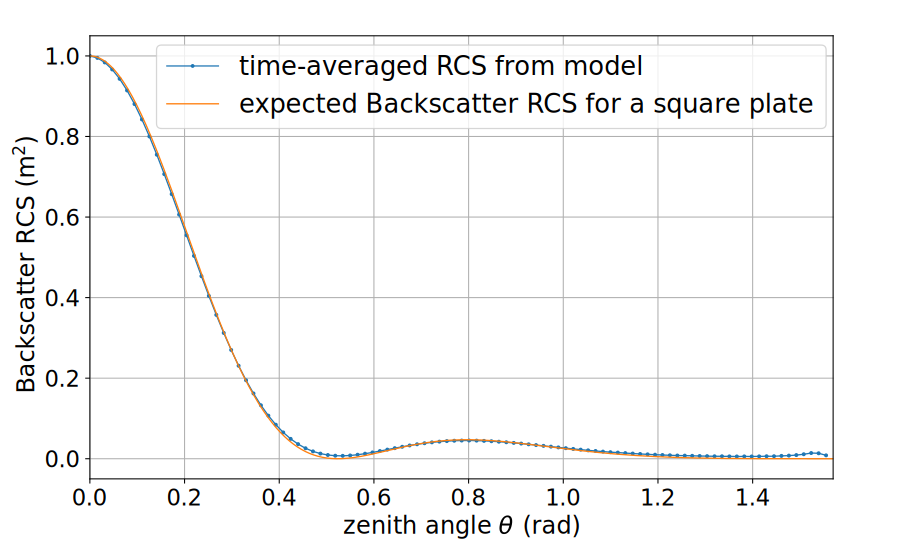
\includegraphics[width=0.8\textwidth]{images/plots/short_2D_cloud_rcs_backscatter_20lambda.pdf}
	\caption{Thin square plate monostatic backscatter. The simulated trend for the normalized RCS (in blue) follows the expected behavior (in orange) as a function of the zenith angle.}
	\label{fig:2D_cloud}
\end{figure}

\noindent The normalized RCS matches the expected behavior of a square plate. This confirms the accuracy of the code. The amplitude was not reproduced since the code is purposed for modeling a material much different from a metal: a cloud. Reproducing the movement of free electrons on a conductive plate is not the main topic of this work, but it can be done describing the electrons with the Thompson scattering cross section.

\section{Rain volumes simulations}
\label{sec:rain_volume_sims}

\noindent All simulations of this work are meant to quantify the power received from scattering by one (Section~\ref{sec:single_raindrop_results}) ore more (Section~\ref{sec:results_portion} and Section~\ref{sec:results_large}) hydrometeors suspended in the atmosphere. The geometry and power transmitted do not reproduce any specific event but are rather a representative of a generic phenomenon of hydrometeor scattering. Specific detector conditions are a topic of upcoming work. \\

\noindent Astroparticle observatories monitor the VHF and UHF spectrum ($f \in$ [30 MHz, 3 GHz]), a range shared with numerous powerful anthropogenic sources. These include FM radio stations and digital television broadcasts, which typically radiate at effective isotropic radiated powers (EIRP)\footnote{In telecommunications, the term EIRP refers to the power that would have to be radiated by an hypothetical isotropic antenna to achieve the same signal level in the direction of maximum radiation of an antenna.} of tens to hundreds of kilowatts. Airborne radars can reach 1 MW, while ground based installations often emit tens of MW. The most powerful radars on Earth are the over-the-horizon (OTH) ones, which use skywave propagation for long-range surveillance and early warning. Their typical EIRP ranges from tens of MW to over a GW. While radio and TV are continuous, narrowband sources, radars emit high-power wideband bursts with long quiet periods.\\

\noindent Within the MARES framework, the EIRP in the direction of the target, is represented by $P\text{eff}=P_{\text{T}}\times G_{\text{T}}$, where $G_{\text{T}}$ is the antenna gain, assumed one in this work. \\

\noindent We have detailed in Section~\ref{sec:final_adaptation} how, given a scattering event, parameters like the RCS and the voltage received are retrieved for each moment in time. The following results represent the average in time of these values. For a pure, unmodulated continuous wave, the average received voltage ($P_{\text{cw}}$) must exceed the noise floor of the instrument to be measurable. This is the parameter we use to estimate the detectability of hydrometeor scattering.\\

\noindent To understand or reproduce the hereby presented results one can keep in mind the following geometry:

\begin{itemize}
	\item [-] One transmitter located at the origin $(x, y, z) = (0, 0, 0)$ m;
	\item [-] One receiver positioned at increasingly larger distances from the transmitter $(x, y, z)$ =  (0 m, $y_{\text{R}}$, 0 m), tuned on the same frequency as the transmitter;
	\item [-] One target (raindrop or rain volume) suspended in the atmosphere $(x, y, x)$ =  (0 m, $y_{\text{tg}}$, 600 m).
\end{itemize}  

\noindent Without loss of generality, we make the following choices: the scattering plane is the $xy$-plane, therefore $x_{\text{tg}} = 0$ m. Furthermore, since it doesn't limit the number of scattering angles considered, the target is always positioned in the middle to simplify calculations: $\alpha = (\pi - \theta)/2$, where $\alpha$ is the angle between the vertical and $\vec{R}_{\text{T}}$, for a graphical representation, see Figure \ref{fig:geometry2}. \\

\begin{figure}[!t]
	\centering
	\includegraphics[width=0.8\textwidth]{images/geometry_2.png}
	\caption{Geometry of the simulation. The Earth's reference frame is portrayed in purple, along with two antennas and an elevated target in symmetrical position. The scattering angle $\theta$ is related to $\alpha$ according to $\alpha = (\pi - \theta)/2$.}
	\label{fig:geometry2}
\end{figure}

\noindent Target and receiver positions $y_{\text{tg}}$ and $y_{\text{R}}$ are varied from 0 to $\tan(\alpha)\cdot 600$ m and 0 to $2\tan(\alpha)\cdot 600$ m respectively, covering scattering angles $\theta \in [\pi, 0)$.

\newpage

\subsection{Results for a single raindrop}
\label{sec:single_raindrop_results}

\begin{figure}[!h]
	\centering
	\begin{subfigure}{0.7\textwidth}
		\centering
		\includegraphics[width=\textwidth]{images/plots/single_sphere_bistatic_surface_plot.pdf}
		\caption{Surface plot.}
	\end{subfigure}
	\hfill
	\begin{subfigure}{0.7\textwidth}
		\centering
		\includegraphics[width=\textwidth]{images/plots/single_sphere_bistatic_heatmap.pdf}
		\caption{Heatmap.}
	\end{subfigure}
	\caption{Radar cross section of a water sphere with $D = 1.69$ mm.}
	\label{fig:single_sphere}
\end{figure}

\noindent The MARES results for scattering from a single water sphere are represented in Figure~\ref{fig:single_sphere}. The full 3D surface plot of the $\sigma_{RCS}$ shows the angular dependency expected from theory (Figure~\ref{fig:angular_distribution}) and an absolute value consistent with the order of magnitude obtained from Equation \ref{eq:effective_area}, with size of droplet $D = 2a = 1.69$ mm and wavelength $\lambda$ = 1 m.

\newpage

\subsection{Results for a small spherical rain volume}
\label{sec:results_portion}

\begin{figure}[!h]
	\centering
	\includegraphics[width=0.7\textwidth]{images/plots/5m_sphere_heatmap_betterresolution_test2_cut.pdf}
	\caption{Radar cross section of a spherical rain volume of 5 meters radius containing raindrops with $D = 1.69$ mm and density 0.1 $\text{g}/\text{cm}^{3}$.}
	\label{fig:5m_sphere_better_resolution}
\end{figure}

\noindent A sphere of 5 m radius contains multiple raindrops. In the case of raindrops of 1.69 mm diameter we found that the density is around 40 raindrops$/\text{m}^{3}$. The response of a spherical volume of that many raindrops is depicted in Figure~\ref{fig:5m_sphere_better_resolution}. \\


\noindent For a target with dimensions comparable to the wavelength, constructive and destructive interference phenomena arise. These interference effects are highly dependent on the angular configuration, leading to a Radar Cross Section (RCS) that can either exceed or fall below that of an isolated droplet. \\

\noindent As mentioned in Section~\ref{sec:small_cloud}, the values from this plot are tabulated to be used in the next simulations (large rain volume) and overcome computational complexity.

\subsection{Results for a large rain volume}
\label{sec:results_large}

\begin{figure}
	\centering
	\begin{minipage}{0.48\textwidth}
		\centering
		\includegraphics[width=\textwidth]{images/plots/medium_cloud100_5mspheres_300MHz_heatmap_betterresolution.pdf}
		\caption{Radar cross section of a cubic cloud of 100$^{3}$ $\text{m}^{3}$.}
		\label{fig:cube_cloud100}
	\end{minipage}
	\hfill
	\begin{minipage}{0.48\textwidth}
		\centering
		\includegraphics[width=\textwidth]{images/plots/medium_cloud300_5mspheres_300MHz_heatmap_betterresolution.pdf}
		\caption{Radar cross section of a cubic cloud of 300$^{3}$ $\text{m}^{3}$.}
		\label{fig:cube_cloud300}
	\end{minipage}
\end{figure}


\begin{figure}
	\centering
	\begin{minipage}{0.48\textwidth}
		\centering
		\includegraphics[width=\textwidth]{images/plots/medium_cloud500_5mspheres_300MHz_heatmap_betterresolution.pdf}
		\caption{Radar cross section of a cubic cloud of 500$^{3}$ $\text{m}^{3}$.}
		\label{fig:cube_cloud500}
	\end{minipage}
	\hfill
	\begin{minipage}{0.48\textwidth}
		\centering
		\includegraphics[width=\textwidth]{images/plots/medium_cloud700_5mspheres_300MHz_heatmap_betterresolution.pdf}
		\caption{Radar cross section of a cubic cloud of 700$^{3}$ $\text{m}^{3}$.}
		\label{fig:cube_cloud700}
	\end{minipage}
\end{figure}

\noindent For the larger volume of rain, the shape of a cube is taken into consideration. The scattering points are placed into a three-dimensional matrix structure that extends for $L$ in all directions. Each scattering point is associated with a RCS from the table retrieved in Section~\ref{sec:results_portion}, using the procedure explained in Section~\ref{sec:big_cloud}. From Figures~\ref{fig:cube_cloud100} to~\ref{fig:cube_cloud700} the RCS of a cubic cloud with variable $L$ is presented. $L$ runs from 100 m to 700 m.\\

\noindent The RCS grows with the effective size of the cloud. The effective size being the intersection between the cloud and the beamwidth of the signal. Both of these are kept generic throughout this study. Figure~\ref{fig:sizes} represents the variation of the RCS as a function of the effective size.\\

\newpage
\begin{figure}
	\centering
	\includegraphics[width=0.7\textwidth]{images/plots/rcs_sizes_all_thetas_phi=1.5.pdf}
	\caption{Radar cross section as a function of the effective size of the rain volume. The dependence is portrayed for different values of $\theta$, and a fixed $\phi = 45^{\circ}$.}
	\label{fig:sizes}
\end{figure}

\noindent As expected, the RCS grows with the volume illuminated by the transmitter. However, the growth is limited by destructive interference phenomena within the volume. Therefore, it is expected that beyond certain critical size, further expansion of the simulated volume returns a negligible effect on the RCS. The precise determination of this threshold was precluded by prohibitive computational constraints.\\

\noindent For the following analysis, a cloud the size of 500$^{3}$ $\text{m}^{3}$ is considered, keeping in mind that in any specific case the RCS can vary by few orders of magnitude depending on the beamwidth and the height of the rain volume. \\

\noindent The analysis proceeds by fixing the angular coordinates $\theta$ and $\phi$ to isolate the dependence of the detected signal on other parameters. These are, the frequency of the signal, the distances $R_{\text{T}}$ and $R_{\text{R}}$ and the power transmitted. \\

\noindent Firstly, we notice that the only parameter that influences the RCS other than the effective size, is the frequency of the signal, therefore it is insightful to plot the reflectivity factor (RCS/Volume) as a function of frequency (see Figure~\ref{fig:RCS_freq}).\\

\begin{figure}
	\centering
	\includegraphics[width=0.7\textwidth]{images/plots/RCSlambda_5mspheres.pdf}
	\caption{Reflectivity factor of a rain volume as a function of frequency. There is a linear dependency between reflectivity and frequency in the UHF range.}
	\label{fig:RCS_freq}
\end{figure}

\noindent The reflectivity varies of two orders of magnitude along the UHF range. The choice of a specific frequency in this range changes the detected signal only by one order of magnitude at most, since the voltage received depends on $\sqrt{\sigma_{\text{RCS}}}/f$ (see Equation~\ref{eq:code_equation_voltage}).\\

\noindent In Figure \ref{fig:R1R2} is quantified the voltage received from a signal with EIRP of $10^{3}$ W at 900 MHz, scattered by a 500$^{3}$ $\text{m}^{3}$ cloud. Fixed these three variables, the voltage depends on the RCS of the target (determined by the hydrometeors' type, density and distribution) and the distances between the target and the antennas, $\text{R}_{\text{T}}$ and $\text{R}_{\text{R}}$.  \\

\begin{figure}
	\centering
	\includegraphics[width=0.6\textwidth]{images/plots/900MHz_5mspheres_R1R2.pdf}
	\caption{Reflected voltage from a 500$^{3}$ $\text{m}^{3}$ convective rain volume. A radiated signal with EIRP = $10^{3}$ W at 900 MHz is considered.}
	\label{fig:R1R2}
\end{figure}

\noindent As expected, the dependence from $\text{R}_{\text{T}}$ and $\text{R}_{\text{R}}$ is symmetric between transmitter and receiver. It is interesting to notice that the reflection is more effective when $y_{\text{tg}}$ is the middle point between the antennas ($\text{R}_{\text{T}} = \text{R}_{\text{R}}$). \\

\noindent As a rule of thumb, we consider the minimum voltage that can be significant for a typical radar system is in the order of magnitude of $\mu V$. The exact threshold for detection will greatly depend on the instrumentation and trigger method of each particular radio detector. Therefore, the analysis was constrained to ranges where $\text{R}_{\text{R}}+\text{R}_{\text{T}}<500$ km. Outside of this limit, the predicted signal strength would fall below the detectable threshold adopted here. \\

\noindent The last variable to be considered is the transmitted power, which effectively is also influenced by the gain of the transmitter antenna. The results of varying the effective power transmitted ($\text{P}_{\text{T}}\text{G}_{\text{T}}$), while keeping fixed $\text{R}_{\text{R}} = 0.5$ km are depicted in Figures~\ref{fig:PTR2_100} and~\ref{fig:PTR2_900}. \\

\begin{figure}
	\centering
	\begin{minipage}{0.48\textwidth}
		\centering
		\includegraphics[width=1\textwidth]{images/plots/100MHz_5msphere_PTR2.pdf}
		\caption{Radiated signal at 100 MHz.}
		\label{fig:PTR2_100}
	\end{minipage}
	\hfill
	\begin{minipage}{0.48\textwidth}
		\centering
		\includegraphics[width=1\textwidth]{images/plots/900MHz_5msphere_PTR2.pdf}
		\caption{Radiated signal at 900 MHz.}
		\label{fig:PTR2_900}
	\end{minipage}
	\caption{Received voltage from a 500$^{3}$ $\text{m}^{3}$ convective rain volume.}
\end{figure}

\noindent The received voltage from hydrometeor scattering is not negligible for distances between the antennas up to 500 km, admitting EIRP = 1 kW at least. This is true for both extremes of the UHF range. Another interesting remark is that the effective size of the rain volume could change the received voltage by one order of magnitude. This consideration is obtained remembering the variability of the RCS over the sizes in Figure~\ref{fig:sizes} and  the square root dependence from $\sigma_{\text{RCS}}$ in Equation~\ref{eq:code_equation_voltage}. \\

\noindent Figures from~\ref{fig:t_7_p_90} to~\ref{fig:t_180_p_90} show the variability of the received voltage with geometry. In each plot a radiated signal at 900 MHz is considered. \\

\begin{figure}
	\centering
	\begin{minipage}{0.48\textwidth}
		\centering
		\includegraphics[width=\textwidth]{images/plots/900MHz_5msphere_PTR2.pdf}
		\caption{Reflected voltage from a 500$^{3}$ $\text{m}^{3}$ rain volume. The geometry is fixed at: $\theta = 7^{\circ}$, $\phi = 90^{\circ}$.}
		\label{fig:t_7_p_90}
	\end{minipage}
	\hfill
	\begin{minipage}{0.48\textwidth}
		\centering
		\includegraphics[width=\textwidth]{images/plots/300MHz_5msphere_PTR2_t14_p90.pdf}
		\caption{Reflected voltage from a 500$^{3}$ $\text{m}^{3}$ rain volume. The geometry is fixed at: $\theta = 14^{\circ}$, $\phi = 90^{\circ}$.}
		\label{fig:t_14_p_90}
	\end{minipage}
\end{figure}


\begin{figure}
	\centering
	\begin{minipage}{0.48\textwidth}
		\centering
		\includegraphics[width=\textwidth]{images/plots/300MHz_5msphere_PTR2_t90_p90.pdf}
		\caption{Reflected voltage from a 500$^{3}$ $\text{m}^{3}$ rain volume. The geometry is fixed at: $\theta = 90^{\circ}$, $\phi = 90^{\circ}$.}
		\label{fig:t_90_p_90}
	\end{minipage}
	\hfill
	\begin{minipage}{0.48\textwidth}
		\centering
		\includegraphics[width=\textwidth]{images/plots/300MHz_5msphere_PTR2_t180_p90.pdf}
		\caption{Reflected voltage from 500$^{3}$ $\text{m}^{3}$ rain volume. The geometry is fixed at: $\theta = 180^{\circ}$, $\phi = 90^{\circ}$.}
		\label{fig:t_180_p_90}
	\end{minipage}
\end{figure}

\noindent It is possible to conclude that, if the geometry is not favorable, such as in the case of Figure~\ref{fig:t_90_p_90}, the range where hydrometeor scattering is relevant restricts to $R_{\text{T}}+ R_{\text{R}}\le 50$ km and transmitted effective power of at least 1 kW. 
